% \documentclass[11pt,a4paper]{scrartcl}
\documentclass[twoside,10pt,a4paper]{article}
\setlength{\parindent}{0em}
\setlength{\parskip}{1.5em}
\bibliographystyle{apalike}


\renewcommand{\familydefault}{\sfdefault}

\newenvironment{notes}[1][\unskip]{%
\par
\noindent
\textcolor{blue}{\bfseries{Notes - } #1:}
\\ \color{blue}}
{}

\newenvironment{followup}[1][\unskip]{%
\par
\noindent
\textcolor{red}{\bfseries{Follow-up - } #1!!!}
\\ \color{red}}
{}

\newenvironment{question}[1][\unskip]{%
\par
\noindent
\textcolor{orange}{\bfseries{Question - } #1???}
\\ \color{orange}}
{}

\usepackage{mystyle}
% Document Layout
% ---> Document geometry - current setting is set to A4 with relatively narrow margins
\geometry{
  a4paper,
  total={210mm,297mm}, % A4 paper measurement
  left=20mm,
  right=20mm,
  top=25mm,
  bottom=25mm
  }
% ---> Document header and footer setting
\pagestyle{fancy}
\fancyhead[LE,RO]{\leftmark} % Refer to Section/chapter/part on the upperroght of the heading
\fancyhead[RE,LO]{}
\fancyfoot[CE,CO]{}
\fancyfoot[LE,RO]{Page \thepage \, of \pageref{LastPage}} % Print current page and total page number centered in the footer.
% ---> Header and footer horisontal line borders
\renewcommand{\headrulewidth}{1pt}
\renewcommand{\footrulewidth}{0.5pt}

% \definecolor{cell-lghtGry}{RGB}{200,200,200}
%\colorlet{Purple}{blue!40!red}
%\colorlet{Blue}{blue}

\restylefloat{figure}
\restylefloat{table}

% Typesetting code snippets
% The code snippet typesetting below is based on https://www.latextemplates.com/template/code-snippet
% Original Author: This template was created for LaTeXTemplates.com by vel@latextemplates.com
\definecolor{DarkGreen}{rgb}{0.0,0.4,0.0} % Comment color
%\definecolor{highlight}{RGB}{255,251,204} % Code highlight color
\definecolor{highlight}{RGB}{204,255,229} % Code highlight color
\definecolor{Gray}{RGB}{224,224,224}
\definecolor{Purple}{RGB}{255,0,255}
\definecolor{Blue}{RGB}{0,0,255}

\lstdefinestyle{Style1}{ % Define a style for your code snippet, multiple definitions can be made if, for example, you wish to insert multiple code snippets using different programming languages into one document
language=Perl, % Detects keywords, comments, strings, functions, etc for the language specified
backgroundcolor=\color{highlight}, % Set the background color for the snippet - useful for highlighting
basicstyle=\footnotesize\ttfamily, % The default font size and style of the code
breakatwhitespace=false, % If true, only allows line breaks at white space
breaklines=true, % Automatic line breaking (prevents code from protruding outside the box)
captionpos=b, % Sets the caption position: b for bottom; t for top
commentstyle=\usefont{T1}{pcr}{m}{sl}\color{DarkGreen}, % Style of comments within the code - dark green courier font
deletekeywords={}, % If you want to delete any keywords from the current language separate them by commas
%escapeinside={\%}, % This allows you to escape to LaTeX using the character in the bracket
firstnumber=1, % Line numbers begin at line 1
frame=single, % Frame around the code box, value can be: none, leftline, topline, bottomline, lines, single, shadowbox
frameround=tttt, % Rounds the corners of the frame for the top left, top right, bottom left and bottom right positions
keywordstyle=\color{Blue}\bf, % Functions are bold and blue
morekeywords={}, % Add any functions no included by default here separated by commas
numbers=left, % Location of line numbers, can take the values of: none, left, right
numbersep=10pt, % Distance of line numbers from the code box
numberstyle=\tiny\color{Gray}, % Style used for line numbers
rulecolor=\color{black}, % Frame border color
showstringspaces=false, % Don't put marks in string spaces
showtabs=false, % Display tabs in the code as lines
stepnumber=5, % The step distance between line numbers, i.e. how often will lines be numbered
stringstyle=\color{Purple}, % Strings are purple
tabsize=2, % Number of spaces per tab in the code
}

% Create a command to cleanly insert a snippet with the style above anywhere in the document
\newcommand{\insertcode}[2]{\begin{itemize}\item[]\lstinputlisting[caption=#2,label=#1,style=Style1]{#1}\end{itemize}} % The first argument is the script location/filename and the second is a caption for the listing


\pagenumbering{roman}

\begin{document}

  % title ans pharagraps section
  \begin{titlepage}
  \begin{center}


      {\bfseries{\Huge{Deliverable: Analysis of Individual Criteria}}}

    
      {\bfseries{\LARGE{IT Infrastructure Maturity}}}


      {\Large{by}}

    \begin{author}
      \author{\Large{Dale P. Bada}}
    \end{author}


    \vspace*{2.5cm}
    Submitted for Assessment in


    \begin{title}
        \title{\bfseries{\huge{UC1ST1103 - Studio 1}}}
    \end{title}

    \vspace*{2.5cm}
    at


    \Large{Noroff University Collegge}

    \vfill


    \begin{figure}[h!]
      \centering
      
\includegraphics[height=50pt]{Noroff-Logo.png}
    \end{figure}


  \end{center}
\end{titlepage}

  

  % \frontmatter
  % front page, title, table of content etc. will have separate page numbering.
  \tableofcontents
  
  \newpage

  % \listoffigures % uncomment to create list of figures
  % \listoftables % uncomment to create list of tables

  % main document will be rendered with the files listed in this section
  % \mainmatter

  \newpage
  \pagenumbering{arabic}
  \setcounter{page}{1}
  \section{Introduction}

{\huge{Course: UC1PR2101 Programming and Databases}}

S02-PR2-2020

\subsection{Key dates}

\begin{tabular}{r @{} c}
    Duration: & 6 weeks\\
    Start: & 2021-01-04\\
    End: & 2021-02-15\\
    Formative assessment: & TBD\\
    Assessment 1 - Submission date: & TBD\\
    Assessment 2 - Submission date: & TBD\\
\end{tabular}

\subsection{Course Tutors}

\begin{tabular}{r @{} l}
    Course leader: & Johan Van Niekerk\\
    Course lecturer: & Rayne Reid\\
    Course tutor: & Konstantin Lenchik\\
    course tutor: & Mariya Chirchenkova\\
    Support tutor: & Sohail Naseem (KRS)\\
    Support tutor: & Arash Mithraian (OSL)\\
\end{tabular}

\subsubsection{Study goals}

\begin{itemize}
    \item Working with database (SQLite)
        \begin{itemize}
            \item Acquire fundamental skill about working with databases
            \item How to design as simple normalized database
            \item Understand database storage and data structure
            \item Understand database Normalization
            \item Be able to query and interface with databases
            \item How to script and automate database connection, mangagement and datamining
            \item Automate data manipulation and analysis, generating reports and statitics etc on data in databases, dataframes etc.
            \item Understanding and being able to manage and  work with databases is therefore key to the field of CyberSecurity.
        \end{itemize}
\end{itemize}


  \newpage
  % This is a section template for reflective journal


% Remove or comment out this whole environment when using this template.
{\begin{center}
    \textcolor{red}{\Huge{THIS IS AN EMPTY SECTION TEMPLATE}}

    \begin{tabular}{r @{: } p{80mm}}
        {\textcolor{blue}{Blue text}} &  Help text. Short description of how to use an environment or a section in the template.\\
        <<{\emph{text placeholder}}>> & Text between angle brackets are placeholders. Indicates a string to be replaced with input text.\\
        Normal text/black fonts & Real note/example text, how the section is intended to be used.
    \end{tabular}

\end{center}


% ----> Header informaton section - Start
\section{Lesson <<{\emph{number}}>>: <<{\emph{Lesson topic}}>>}

{\textcolor{blue}{Replace the double angle brackets with the lesson number and name.}}

Original URL: <<{\emph{link to the original blog post on the Moodle blog}}>>

{\textcolor{blue}{Replace the double angle brackets with the URL to the reflective journal blog.}}
% <---- Header informaton - End


% ----> Main reflective subsection - Start
% ----| Write reflective thoughts on the topic in general. |----
\subsection{Reflection on the days lecture and tutorial}

{\textcolor{blue}{Add critical reflective thoughts about your learning experiences. Delete this text}}

{\bfseries{Lesson/Topic Objectives  Study Plan:}}
\begin{itemize}
    \item Identify the basic components of a relational model
    \item Understand ERD
    \item Understand data models
    \item Understand data modeling, its objectives of storing and managing, real word data. Data modeling entails organizing, structuring and utilizing stored data for optimized storage, accessibility, searchability and security.
\end{itemize}
% <---- Main reflective subsection - End

% ----> Main reflective subsection - Start
% ----| Write reflective thoughts on a specific reflective topic. |----
\subsection{Reflection Topics}

{\textcolor{blue}{When there are guided topics add them as sub-headings and include your critical discussion of the topic(s)}}

<<{\emph{\blindtext[1]}}>> % Example text, comment out or remove this line.

<<{\emph{\blindtext[1]}}>> % Example text, comment out or remove this line.

\subsubsection{Provided topic 1}

{\textcolor{blue}{topic 1 example reflective discussion}}

<<{\emph{\blindtext[1]}}>> % Example text, comment out or remove this line.

<<{\emph{\blindtext[1]}}>> % Example text, comment out or remove this line.

\subsubsection{Provided topic 2}

{\textcolor{blue}{topic 2 example reflective discussion}}

% <---- Main reflective subsection - End



% ----> Key Take-Away subsection - Start
% ----| Write Itemized notes regarding the lesson topic. |----
\subsection{Key Take-Away}

\begin{table}[H]
    \begin{tabular}{r @{: } p{40mm}}
        Lesson date & {\emph{<<yyyy mm dd>>}} \\
        Date taken & {\emph{<<yyyy mm dd>>}} \\
        Revisited & <<{\emph{comment or yyyy mm dd}}>> \\
    \end{tabular}
\end{table}

{\textcolor{blue}{This subsection outlines key information from the day's lesson in bullet points.}}

\begin{enumerate}\itshape
    \item <<Main Item 1
    \begin{enumerate}
        \item sub item 1 1
        \item sub item 1 2
        \item sub item 1 3
        \item sub item 1 4
        \item sub item 1 5
        \item sub item 1 6
    \end{enumerate}
    \item Main Item 2
    \begin{enumerate}
        \item sub item 2 1
        \item sub item 2 2
        \item sub item 2 3
        \item sub item 2 4
    \end{enumerate}
    \item Main Item 3
    \item ..
    \item .>>
\end{enumerate}


\subsection{Lessons Learned}

{\textcolor{blue}{This subsection summarizes the day's lesson topic.}}

{\bfseries{Bold heading}}

<<{\emph{\blindtext[2]}}>>


{\bfseries{Glossary:}}

{\textcolor{blue}{Expand and elaborate on new words, expressions and topic terminology with a glossary list.}}

\begin{table}[H]\label{tab:glossary}
    \begin{tabular}{p{40mm} | p{120mm}}
        {\bfseries{Key Word/Expression}} & {\bfseries{Elaboration/Comment}}\\ \hline
        <<{\emph{Input}}>> & <<{\emph{Input}}>>\\ \hline
    \end{tabular}
\end{table}

% <---- Lessons Learned subsection - End



% ----> Action-Point subsection - Start
% ----| To-do list to complete the day's lesson topic. |----
\subsection{Action Points - Further Reading/Enquiry}

{\textcolor{blue}{To-do list relevant to complete/expand on the lesson topic.}}

\begin{adjustbox}{max width=\textwidth}
    \begin{tabular}{c|l|l|c|l}
        {\bfseries{Act Pnt}} & {\bfseries{To-do description}} & {\bfseries{Assigned to}} & {\bfseries{Target date}} & {\bfseries{Comment/Status}} \\
        \hline
        1 & <<{\emph{Task name/description}}>> & <<{\emph{Task owner}}>> & <<{\emph{Deadline yyyy-mmm-dd}}>> & <<{\emph{Comments or status}}>> \\ \hline
        2 & <<{\emph{Task name/description}}>> & <<{\emph{Task owner}}>> & <<{\emph{Deadline yyyy-mmm-dd}}>> & <<{\emph{Comments or status}}>> \\ \hline
    \end{tabular}
\end{adjustbox}

% <---- Action-Point subsection - End



% ----> Other source materials subsection - Start
% ----| A list of materials not directly provided via the course books/distributed by lecturers for the day's lesson topic. |----
\subsection{Other source materials} 

{\textcolor{blue}{External course related material. Insert book title, ISBN, URL etc. }}

\begin{table}[H]\label{tab:sources}
    \begin{tabular}{p{10mm} | p {47mm} | p{100mm}}
        {\bfseries{Item num.}} & {\bfseries{Resource Type}} & {\bfseries{Source description, Book title, URL, etc.}}\\
        \hline
        1 & <<{\emph{Input}}>> & <<{\emph{Input}}>>\\ \hline
    \end{tabular}
\end{table}

% <---- Other source materials subsection - end

% ----> Issues Noted and Area of Improvements subsection - Start
% ----| A list of items, after-thought about issues, difficulties (on the subject itself, materials, tools, etc.) working with the day's lesson topic. |----
\subsection{Issues/Solutions Noted and Area of Improvements}

{\textcolor{blue}{Issues noted; what has failed with regards to tools, the lecture itself, missing course material, wrong information or solution in the course assignment etc. Any area of improvement with regards to how previous task has been managed, how to more efficiently proceed with the course personally. Suggestions for improvement suggestions to course leader.}}

\begin{table}[H]\label{tab:issuensolution}
    \begin{tabular}{p{10mm} | p {47mm} | p{100mm}}
        {\bfseries{Item num.}} & {\bfseries{Issue description / Area of Improvement}} & Comments / Solution \\ \hline
        1 & <<{\emph{input}}>> & <<{\emph{input}}>>\\ \hline
    \end{tabular}
\end{table}

% <---- Issues Noted and Area of Improvements subsection - End
  

  \newpage
  \section{Conclusion}

Norway is actually 100\% aligned with the European NIS Directive. However, there is little evidence that Norway has identified its \acrshort{oes} according to EU's guideline.

\begin{followup}
  Outline the complexities navigaating the different documents and legislations in the EU and Norway.

  There are many stakeholders, authorities and agencies, that regulates and sets policies. Often with over lapping responsibilities and objectives. Making passing policies and implmenting policies complicated.
  
  Many Member states must adhere to and align both National and EU NIS Directive when establishing or revising their NCSS. Again, adding to complexity and GAPS.

  A mix and differing definitions and terminologies are bing used and are not always aligned with each other. Making translation of policies tricker. There is a lack of formal and standardised definitons on most cases.
\end{followup}


% \includesvg{tex/Studio_1_Activity_Diagram.svg}
% 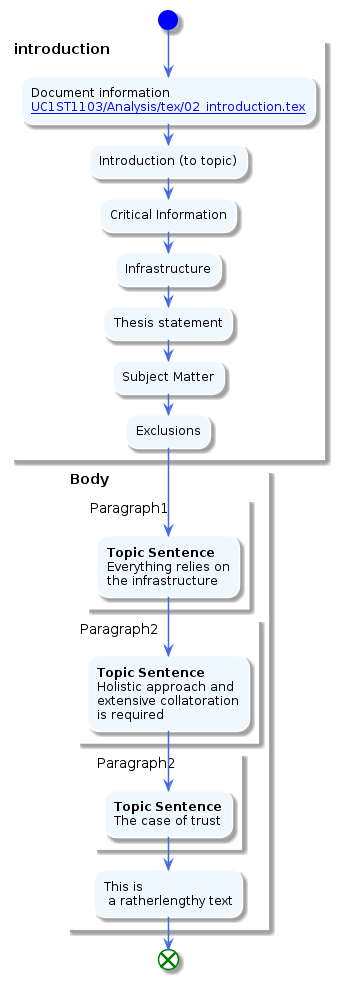
\includegraphics{tex/Studio_1_Activity_Diagram.png}





  \newpage
  \appendix
  \section{Appendix}

This is the appendix

  % bibliography
  \newpage
  % \clearpage
  % \input{tex/06_bibliography.tex}

  \section{Bibliography}
  \printbibliography

\end{document}